\documentclass[../../General.tex]{subfiles}
\begin{document}

\section{Diseño de subsistema de orientación de piranómetro}

\subsection{Descripción general del subsistema}

El subsistema de orientación, mostrado en la Figura \ref{fig:SubsistemaOrientacionCAD}, ejecuta el giro de alabeo (\textit{roll}) de la plataforma que porta el piranómetro. El eje de giro es paralelo a la dirección de avance del robot; de este modo, cuando el robot circula por el pasillo paralelo a las filas de módulos, el giro de alabeo permite igualar la inclinación del sensor con la del plano de los módulos fotovoltaicos. Para sistemas de monitoreo Clase A, la norma IEC 61724-1 exige que los sensores de irradiancia alineados con el plano de los módulos mantengan una tolerancia de $0.5^\circ$ en inclinación y de $1.0^\circ$ en azimut \citep{IEC61724-1_2021}. Este subsistema controla la inclinación; la tolerancia de azimut depende del rumbo del robot respecto a la fila de módulos y no se controla con este subsistema.

El subsistema se monta sobre el de elevación (Sección \ref{sec:subsistema_elevacion}): una viga 2040 del subsistema de orientación se dispone en sentido longitudinal, paralela al avance, y se fija al alma de la pieza en U del subsistema de elevación. El motor NEMA 17 y la caja del tornillo sin fin quedan hacia el frente del robot.

El control de este subsistema corrige únicamente la inclinación lateral (\textit{roll}); no corrige el cabeceo (\textit{pitch}). Como el paralelogramo de elevación traslada la plataforma sin rotarla, el \textit{pitch} del sensor es el del chasis. Por ello, la medición se realiza solo en tramos casi planos. El MPU-6050 montado en el eje basculante mide el vector gravedad en tres ejes, de modo que entrega tanto el \textit{roll} como el \textit{pitch} de la plataforma, y es la medición más directa para verificar esa condición.

Para una plataforma inclinada un ángulo $\beta$ alrededor del eje longitudinal, un \textit{pitch} $p$ desvía el azimut de la normal del sensor en $p \cot\beta$ aproximadamente. Con la tolerancia de azimut de $1.0^\circ$ de la IEC 61724-1, el \textit{pitch} admisible es $|p| \leq 1.0^\circ \cdot \tan\beta$, cuyos valores se muestran en la Tabla \ref{tab:pitch_admisible_tilt}.

\begin{center}
    \footnotesize
    \begin{xltabular}{0.8\textwidth}{|>{\centering\arraybackslash}X|>{\centering\arraybackslash}X|>{\centering\arraybackslash}X|}
        \caption{\textit{Pitch} admisible según la inclinación de la plataforma\label{tab:pitch_admisible_tilt}} \\
        \hline
        \rowcolor[HTML]{D9E1F2}
        Inclinación $\beta$ & \textit{Pitch} admisible [$^\circ$] & ¿Cumple $\geq 0.2^\circ$? \\ \hline
        \endfirsthead

        \multicolumn{3}{c}%
        {\tablename\ \thetable{} -- Continuación de la página anterior} \\
        \hline
        \rowcolor[HTML]{D9E1F2}
        Inclinación $\beta$ & \textit{Pitch} admisible [$^\circ$] & ¿Cumple $\geq 0.2^\circ$? \\ \hline
        \endhead

        \hline
        \endfoot

        \hline
        \endlastfoot

        $5^\circ$ & $0.087$ & No \\ \hline
        $10^\circ$ & $0.18$ & No \\ \hline
        $12^\circ$ & $0.21$ & Sí ($\beta_{\min}$) \\ \hline
        $18^\circ$ & $0.32$ & Sí \\ \hline
        $30^\circ$ & $0.58$ & Sí \\ \hline
    \end{xltabular}
\end{center}

El límite de \textit{pitch} solo es verificable si supera la incertidumbre con la que se mide. Con la exactitud de $0.1^\circ$ del MPU-6050 tras la calibración y un margen de 2, se exige $1.0^\circ \cdot \tan\beta \geq 0.2^\circ$, lo que da $\beta_{\min} = 11.3^\circ$, que se redondea a $\beta_{\min} = 12^\circ$. Para $\beta \geq 12^\circ$, el subsistema cumple la tolerancia de inclinación y la de azimut de la norma, siempre que el \textit{pitch} del chasis no supere el valor de la Tabla \ref{tab:pitch_admisible_tilt}. Para $\beta < 12^\circ$, solo se verifica la tolerancia de inclinación de $0.5^\circ$ y no se reclama la de azimut: la IEC 61724-1 no fija tolerancia de azimut para sensores horizontales, y a inclinaciones bajas el azimut tiende a no afectar la irradiancia recibida. El margen de 2 y el umbral de $12^\circ$ son criterios de diseño de este trabajo, no valores de la norma. El rango mecánico de $\pm 30^\circ$ no cambia.
% PENDIENTE: confirmar con el texto literal de la IEC 61724-1 (seccion y redaccion) lo dicho sobre azimut en sensores horizontales, y verificar que beta_min = 12 deg no excluya las inclinaciones de las plantas objetivo.

El giro se transmite desde un motor a pasos NEMA 17 mediante un tornillo sin fin y una corona, que se fabrican en torno CNC. La transmisión se autobloquea en reposo, de modo que el peso del sensor y la carga de viento no hacen retroceder el mecanismo. Un sensor inercial MPU-6050, montado en una chapa solidaria al eje, mide el ángulo de alabeo y cierra el lazo de control de posición.

\begin{figure}[H]
	\captionsetup{justification=raggedright, singlelinecheck=false, labelsep=none}
	\caption[Vista isométrica y derecha del subsistema de orientación.]{}
	\textit{Vista isométrica y derecha del subsistema de orientación.} \par\medskip

	\begin{minipage}{0.5\textwidth}
		\centering
		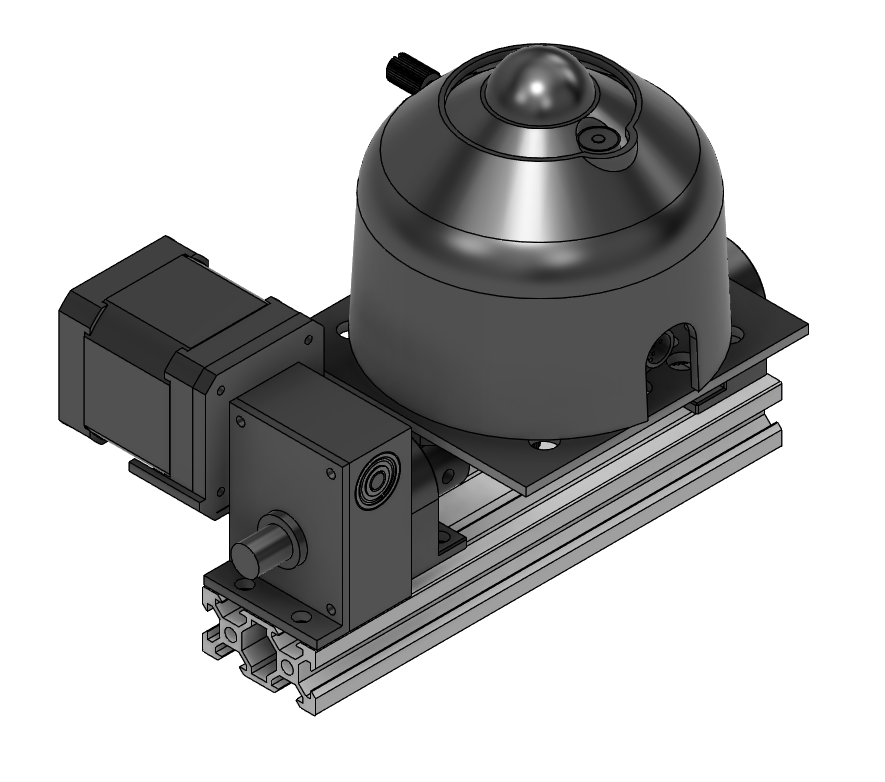
\includegraphics[width=\linewidth]{Recursos/Imagenes/ImagenesDisenoMecanico/MECANISMO_ORIENTACION_ISO1.png}
	\end{minipage}\hfill
	\begin{minipage}{0.5\textwidth}
		\centering
		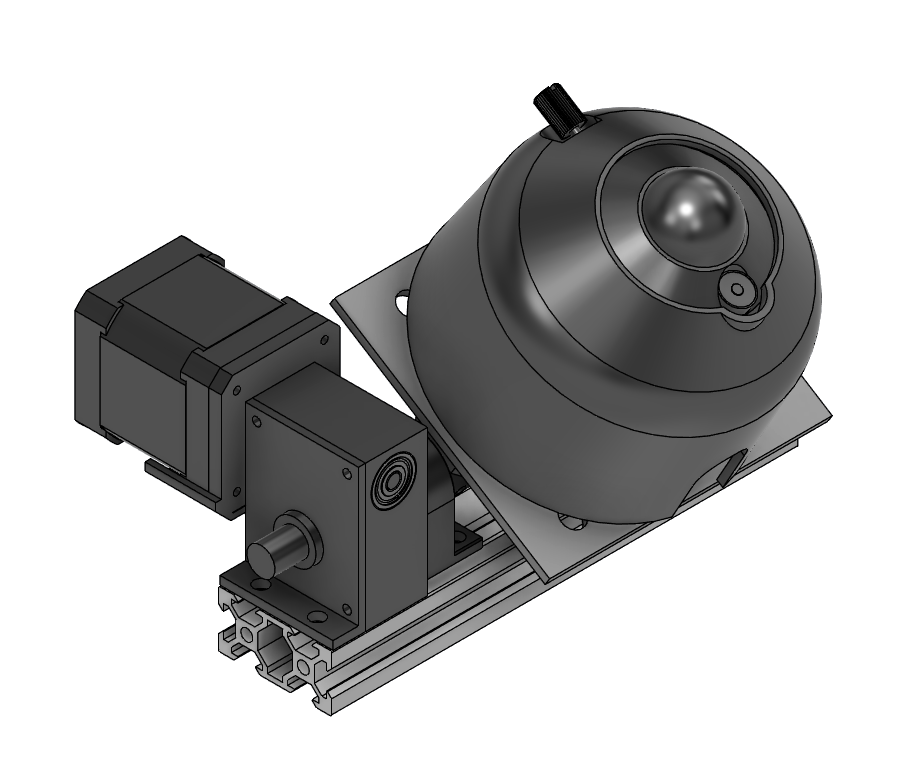
\includegraphics[width=\linewidth]{Recursos/Imagenes/ImagenesDisenoMecanico/MECANISMO_ORIENTACION_ISO2.png}
	\end{minipage}
	\par\medskip

	\raggedright
	\footnotesize \textit{Nota.} Elaboración propia.
	\label{fig:SubsistemaOrientacionCAD}
\end{figure}

\subsection{Planteamiento inicial y parámetros de diseño}

El subsistema debe orientar una plataforma que gira alrededor de un eje central y que soporta el sensor de irradiancia. El diseño debe sostener la carga en cualquier punto de la trayectoria, resistir la carga de viento y alcanzar la tolerancia angular de la norma. Los datos de entrada y las restricciones del análisis se resumen en la Tabla \ref{tab:parametros_diseno_tilt}.

\begin{center}
    \footnotesize
    \begin{xltabular}{\textwidth}{|p{3.5cm}|>{\centering\arraybackslash}p{2.2cm}|>{\centering\arraybackslash}p{2.8cm}|>{\centering\arraybackslash}X|}
        \caption{Datos de entrada y restricciones del subsistema de orientación\label{tab:parametros_diseno_tilt}} \\
        \hline
        \rowcolor[HTML]{D9E1F2}
        Parámetro & Símbolo & Valor & Descripción \\ \hline
        \endfirsthead

        \multicolumn{4}{c}%
        {\tablename\ \thetable{} -- Continuación de la página anterior} \\
        \hline
        \rowcolor[HTML]{D9E1F2}
        Parámetro & Símbolo & Valor & Descripción \\ \hline
        \endhead

        \hline
        \endfoot

        \hline
        \endlastfoot

        \multicolumn{4}{|l|}{\textbf{Carga y plataforma}} \\ \hline
        Masa de diseño del sensor & $m_{\text{carga}}$ & $0.50\text{ kg}$ & Envolvente de piranómetros Clase A de masa $\leq 0.50\text{ kg}$. \\ \hline
        Excentricidad del centro de masa & $d_{\text{cm}}$ & $25\text{ mm}$ & Distancia supuesta entre el eje de giro y el centro de masa del sensor. \\ \hline
        Masa de la plataforma & $m_{\text{plat}}$ & $0.25\text{ kg}$ & Plataforma, soportes y elementos de sujeción. \\ \hline
        Longitud de la plataforma & $L_{\text{plat}}$ & $90\text{ mm}$ & Dimensión de la plataforma en el plano de giro. La placa mide $90\times100\times3\text{ mm}$; los $100\text{ mm}$ van a lo largo del eje basculante. \\ \hline
        \multicolumn{4}{|l|}{\textbf{Movimiento}} \\ \hline
        Rango angular & $\theta$ & $-30^\circ$ a $+30^\circ$ & Barrido total $\Delta\theta = 60^\circ$. \\ \hline
        Tiempo de barrido & $t_{b}$ & $5.0\text{ s}$ & Tiempo para recorrer el barrido completo. \\ \hline
        Fracción de aceleración & $f_{a}$ & $0.25$ & Fracción de $t_b$ en aceleración e igual en desaceleración. \\ \hline
        Tolerancia de inclinación & $\varepsilon_{\text{adm}}$ & $0.5^\circ$ & IEC 61724-1, Clase A \citep{IEC61724-1_2021}. \\ \hline
        \multicolumn{4}{|l|}{\textbf{Transmisión}} \\ \hline
        Módulo axial & $m$ & $1.0\text{ mm}$ & Módulo del par tornillo sin fin y corona. \\ \hline
        Entradas del sin fin & $Z_1$ & $1$ & Número de hilos del tornillo sin fin. \\ \hline
        Dientes de la corona & $Z_2$ & $30$ & Relación de reducción $i = 30$. \\ \hline
        Diámetro exterior del sin fin & $d_{\text{ext}}$ & $14.5\text{ mm}$ & Diámetro de paso $d_w = d_{\text{ext}} - 2m = 12.5\text{ mm}$. \\ \hline
        Ángulo de presión normal & $\phi_n$ & $20^\circ$ & Valor estándar. \\ \hline
        Coeficiente de fricción & $\mu_s$ & $0.15$ & Fricción estática acero--bronce lubricado. \\ \hline
        Juego circunferencial & $j_t$ & $0.28\text{ mm}$ & Referencia de transmisiones comerciales de igual módulo y número de dientes. \\ \hline
        \multicolumn{4}{|l|}{\textbf{Viento (NTE E.020)}} \\ \hline
        Velocidad de diseño & $V$ & $75\text{ km/h}$ & Valor mínimo normativo a $10\text{ m}$ de altura. \\ \hline
        Factor de forma & $C$ & $1.5$ & Elemento con una dimensión corta en la dirección del viento. \\ \hline
        Factor de ráfaga & $f_r$ & $1.2$ & Estructura Tipo 2. \\ \hline
        Área expuesta & $A_{\text{exp}}$ & $0.012\text{ m}^2$ & Área proyectada del sensor y la plataforma. \\ \hline
        Brazo del centro de presión & $h_{\text{cp}}$ & $60\text{ mm}$ & Distancia del centro de presión al eje de giro. \\ \hline
        \multicolumn{4}{|l|}{\textbf{Actuador}} \\ \hline
        Factor de seguridad de torque & $S$ & $1.30$ & Margen para evitar la pérdida de pasos. \\ \hline
        Ángulo de paso y micropasos & -- & $1.8^\circ$, 1/16 & Configuración del motor y del driver. \\ \hline
        Corriente configurada & $I_{\text{set}}$ & $1.40\text{ A}$ & Corriente del driver, $70\%$ de la nominal. \\ \hline
	\end{xltabular}
\end{center}

La masa de diseño de $0.50\text{ kg}$ es una envolvente conservadora. El piranómetro de referencia, el EKO MS-80, tiene una masa de $0.35\text{ kg}$ ($0.41\text{ kg}$ en la versión MS-80S), un diámetro de $96\text{ mm}$ con la pantalla solar y una altura total de $101\text{ mm}$ \citep{eko_ms80_2023}. La envolvente admite cualquier piranómetro Clase A según ISO 9060 \citep{iso9060_2018} de masa igual o menor a $0.50\text{ kg}$. La plataforma es simétrica respecto al eje, por lo que su peso no genera momento. El centro de masa nominal del sensor también está sobre el eje; aun así, se adopta una excentricidad de $25\text{ mm}$ para cubrir desbalances del soporte de interfaz, de los conectores y del cableado lateral.

El rango de $\pm 30^\circ$ cubre la inclinación de módulos fijos en el Perú, cuya latitud varía entre $0^\circ$ y $18^\circ$ S. En latitudes bajas, la inclinación óptima de un módulo fijo es cercana a la latitud del sitio \citep{jacobson2018tilt}. Como el robot circula sobre terreno inclinado, la plataforma debe compensar la suma de la inclinación del módulo y la pendiente del terreno; si esta suma supera $30^\circ$, la configuración queda fuera del rango operativo. Los seguidores solares de un eje alcanzan inclinaciones mayores y no se incluyen en el alcance de este subsistema.

\begin{figure}[H]
	\captionsetup{justification=raggedright, singlelinecheck=false, labelsep=none}
	\caption[Plataforma basculante del piranómetro (izquierda) y mecanismo de transmisión de potencia al eje basculante (derecha).]{}
	\textit{Plataforma basculante del piranómetro (izquierda) y mecanismo de transmisión de potencia al eje basculante (derecha).} \par\medskip

	\begin{minipage}{0.5\textwidth}
		\centering
		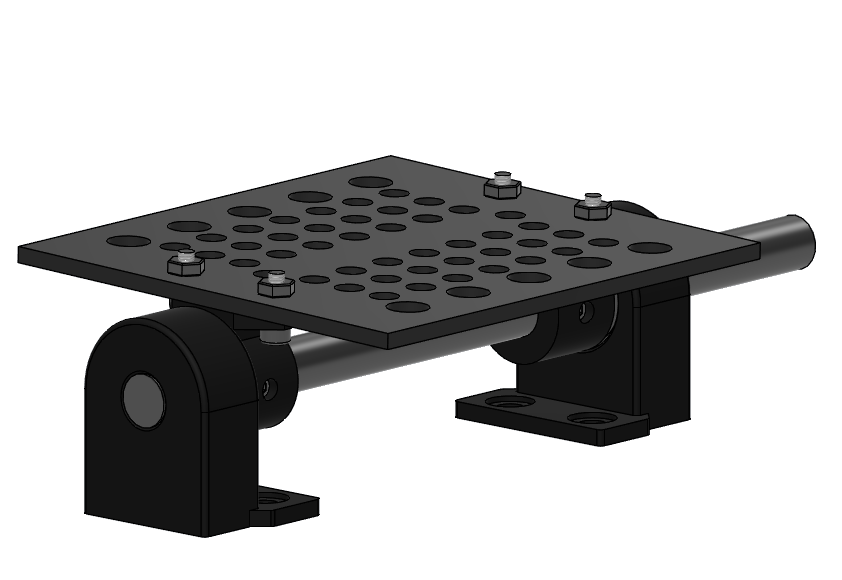
\includegraphics[width=\linewidth]{Recursos/Imagenes/ImagenesDisenoMecanico/SubsistemaOrientacionDisenhoA1.png}
	\end{minipage}\hfill
	\begin{minipage}{0.5\textwidth}
		\centering
		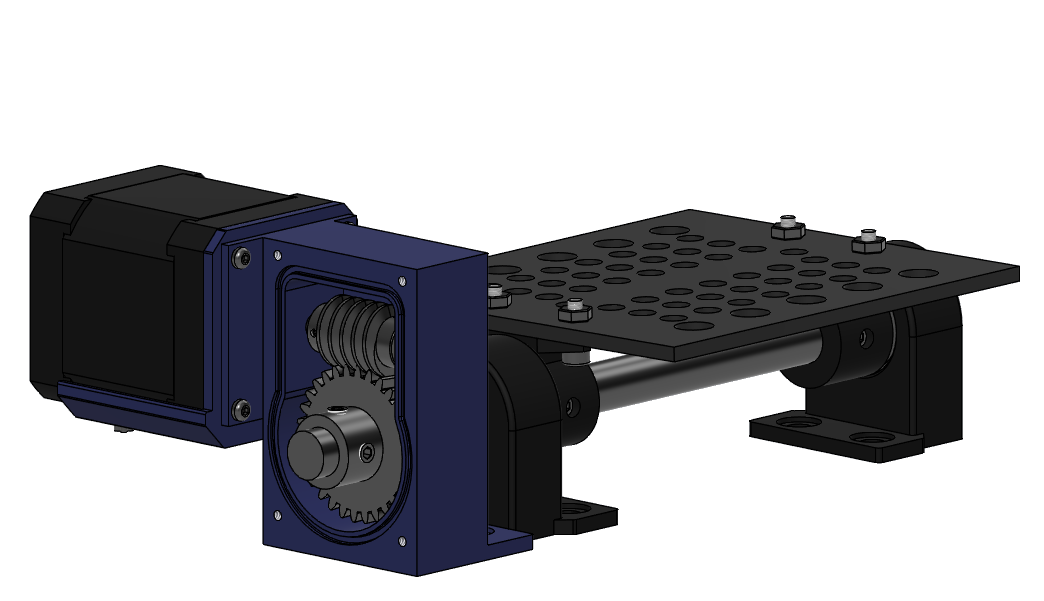
\includegraphics[width=\linewidth]{Recursos/Imagenes/ImagenesDisenoMecanico/SubsistemaOrientacionDisenhoA2.png}
	\end{minipage}
	\par\medskip

	\raggedright
	\footnotesize \textit{Nota.} Derecha, flechas rojas representan la transmisión de potencia desde el motor hacia el eje.
	\label{fig:SubsistemaOrientacionDisenhoA}
\end{figure}

\subsection{Planteamiento cinemático y estático}

\subsubsection{Perfil de movimiento}

La plataforma recorre el barrido de $-30^\circ$ a $+30^\circ$ con un perfil trapezoidal de velocidad: acelera durante un tiempo $t_a = f_a\, t_b$, se mueve a velocidad constante y desacelera durante el mismo $t_a$. La velocidad angular máxima y la aceleración angular son:

\begin{equation}\label{eq:perfil_tilt}
    \omega_{\text{máx}} = \frac{\Delta\theta}{t_b - t_a}, \qquad \ddot{\theta} = \frac{\omega_{\text{máx}}}{t_a}
\end{equation}

Con $t_b = 5.0\text{ s}$ y $f_a = 0.25$, se obtiene $\omega_{\text{máx}} = 0.2793\text{ rad/s}$ ($16.00^\circ/\text{s}$) y $\ddot{\theta} = 0.2234\text{ rad/s}^2$. Con la reducción de 30 a 1, el motor gira a un máximo de $80\text{ rpm}$.

\begin{figure}[H]
	\captionsetup{justification=raggedright, singlelinecheck=false, labelsep=none}
	\caption[Esquematización de movimiento del subsistema de orientación (izquierda) y diagrama de cuerpo libre (derecha).]{}
	\textit{Esquematización de movimiento del subsistema de orientación (izquierda) y diagrama de cuerpo libre del subsistema de orientación (derecha).} \par\medskip

	\begin{minipage}{0.5\textwidth}
		\centering
		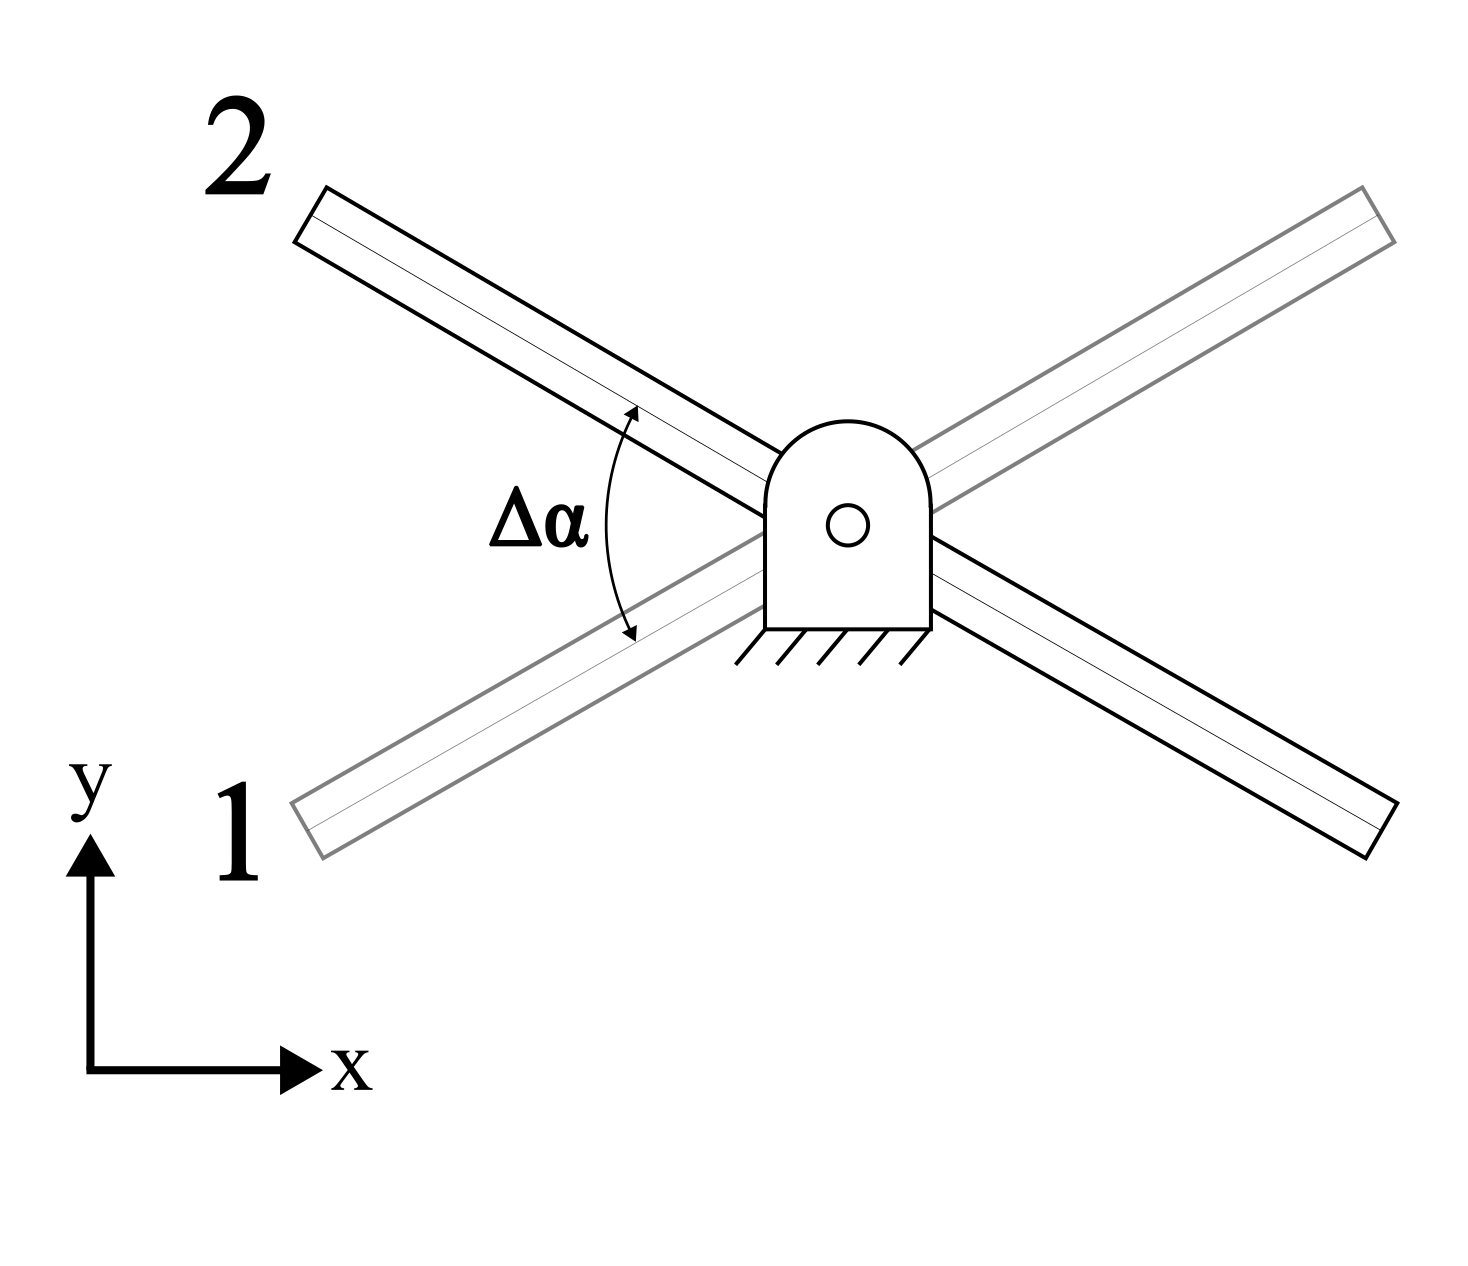
\includegraphics[width=\linewidth]{Recursos/Imagenes/ImagenesDisenoMecanico/Tilt_DCL_1.png}
	\end{minipage}\hfill
	\begin{minipage}{0.5\textwidth}
		\centering
		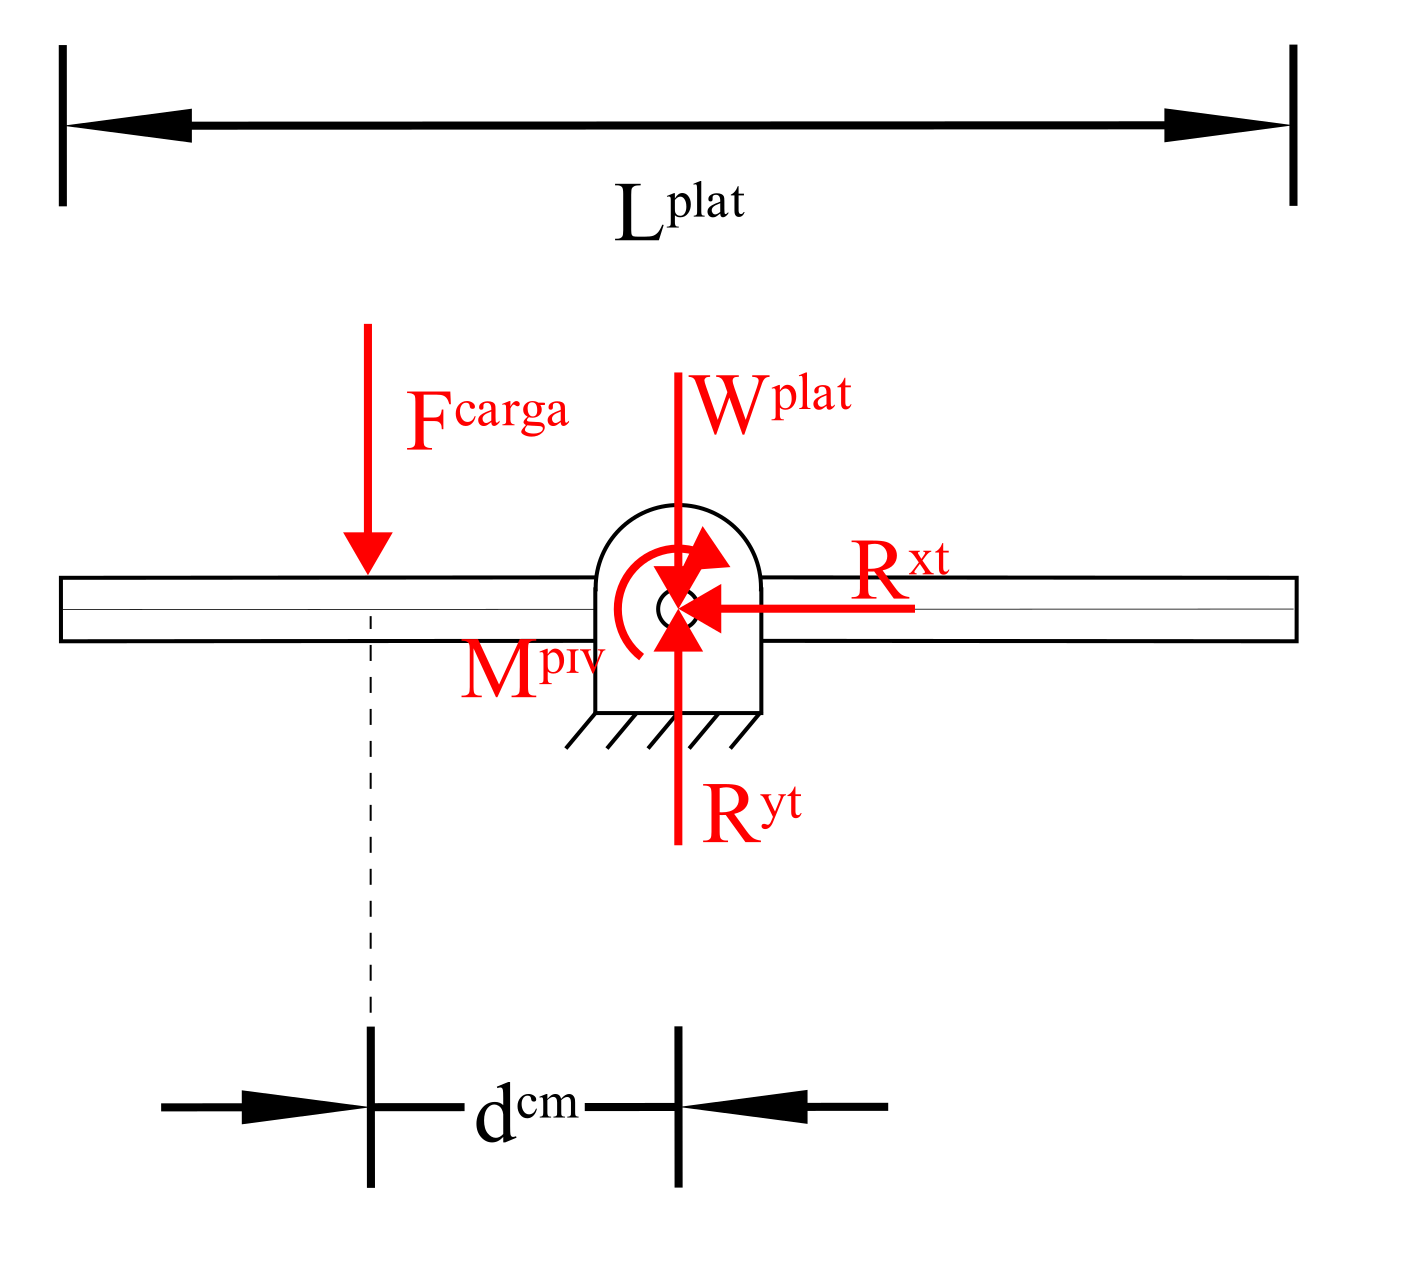
\includegraphics[width=\linewidth]{Recursos/Imagenes/ImagenesDisenoMecanico/Tilt_DCL_2.png}
	\end{minipage}
	\par\medskip

	\raggedright
	\footnotesize \textit{Nota.} Elaboración propia.
	\label{fig:DCLSubsistemaOrientacion}
\end{figure}

\subsubsection{Cargas sobre el eje de giro}

Según el diagrama de cuerpo libre de la Figura \ref{fig:DCLSubsistemaOrientacion}, solo el peso del sensor genera momento gravitacional, porque el peso de la plataforma pasa por el eje. El momento desestabilizador en función del ángulo es:

\begin{equation}\label{eq:Mpiv}
    M_{\text{piv}}(\theta) = m_{\text{carga}}\, g\, d_{\text{cm}} \cos\theta
\end{equation}

Su valor máximo ocurre en $\theta = 0^\circ$ y es $M_{\text{piv}} = 0.1226\text{ N}\cdot\text{m}$.

La carga de viento se calcula con la norma NTE E.020 \citep{nte_e020}. Como el robot no tiene un sitio de operación definido, se adopta la velocidad mínima normativa de $75\text{ km/h}$ a $10\text{ m}$ de altura, que es conservadora para un sensor ubicado a menor altura. La velocidad de diseño a la altura $h$ y la presión de viento son:

\begin{equation}\label{eq:viento_tilt}
    V_h = V \left(\frac{h}{10}\right)^{0.22}, \qquad P_h = f_r \cdot 0.005\, C\, V_h^2
\end{equation}

donde $V_h$ está en km/h y $P_h$ en kgf/m$^2$. El factor de forma $C = 1.5$ corresponde a elementos aislados con una dimensión corta en la dirección del viento, y el factor $f_r = 1.2$ se aplica a las estructuras Tipo 2, sensibles a ráfagas \citep{nte_e020}. La presión resultante es de $50.63\text{ kgf/m}^2$ ($496.5\text{ Pa}$). Sobre el área expuesta de $0.012\text{ m}^2$, la fuerza lateral es $F_v = 5.96\text{ N}$, y con el brazo de $60\text{ mm}$ genera un momento $M_v = 0.3575\text{ N}\cdot\text{m}$ sobre el eje. Este momento es casi tres veces el gravitacional, por lo que el viento es la carga que dimensiona el subsistema.

La fricción de los rodamientos del eje, $T_{\text{rod}} = 0.0201\text{ N}\cdot\text{m}$, se estima con el modelo simplificado de SKF \citep{skf2020bearings}. Proviene casi por completo de los sellos de contacto de los rodamientos.

\subsubsection{Inercia y torque requerido}

La inercia respecto al eje de giro incluye la plataforma, el sensor (con el término de Steiner por su excentricidad), la corona y el propio eje:

\begin{equation}\label{eq:Jtotal_tilt}
    J_{\text{total}} = J_{\text{plat}} + J_{\text{carga}} + J_{\text{corona}} + J_{\text{eje}}
\end{equation}

La plataforma se modela como una placa delgada que gira en su plano de $L_{\text{plat}} = 90\text{ mm}$, de modo que $J_{\text{plat}} = m_{\text{plat}} L_{\text{plat}}^2/12 = 1.688 \times 10^{-4}\text{ kg}\cdot\text{m}^2$. El sensor ($9.015 \times 10^{-4}\text{ kg}\cdot\text{m}^2$) aporta la mayor parte del total, seguido de la plataforma; la corona y el eje contribuyen de forma marginal. La inercia total es $J_{\text{total}} = 1.078 \times 10^{-3}\text{ kg}\cdot\text{m}^2$.

Como la transmisión se autobloquea, el motor siempre debe impulsar la carga, incluso cuando la gravedad o el viento actúan a favor del giro. Por ello, el torque en el eje de salida se calcula sumando los módulos de todos los términos:

\begin{equation}\label{eq:Tout_tilt}
    T_{\text{out}}(t) = M_{\text{piv}}(\theta) + M_v + T_{\text{rod}} + J_{\text{total}} \left|\ddot{\theta}(t)\right|
\end{equation}

El torque requerido en el motor divide el torque de salida por la relación de reducción y la eficiencia estática del engrane, y suma la aceleración de las masas del lado del motor (rotor, tornillo sin fin y acoplamiento):

\begin{equation}\label{eq:Tmotor_tilt}
    T_{\text{motor}}(t) = \frac{S\, T_{\text{out}}(t)}{i\, \eta_s} + S\, J_{\text{m}}\, i \left|\ddot{\theta}(t)\right|
\end{equation}

Se usa la eficiencia estática $\eta_s$ porque el caso crítico de un motor a pasos es el arranque desde el reposo, cuando la fricción del engrane es máxima. La fricción de los rodamientos queda dentro de $T_{\text{out}}$, y la fricción del engrane, dentro de $\eta_s$, de modo que ninguna se cuenta dos veces.

\subsection{Dimensionamiento de componentes}

\subsubsection{Transmisión de tornillo sin fin y corona}

El diámetro del tornillo sin fin es una decisión de diseño, ya que el juego se fabrica a medida. Con un diámetro exterior de $14.5\text{ mm}$, el diámetro de paso es $d_w = 12.5\text{ mm}$, lo que corresponde a un factor diametral $q = d_w/m = 12.5$. El ángulo de avance, el diámetro de paso de la corona y la distancia entre centros son:

\begin{equation}\label{eq:geom_sinfin}
    \lambda = \arctan\!\left(\frac{m\, Z_1}{d_w}\right) = 4.574^\circ, \qquad d_2 = m\, Z_2 = 30\text{ mm}, \qquad a = \frac{d_w + d_2}{2} = 21.25\text{ mm}
\end{equation}

La eficiencia directa (el sin fin impulsa a la corona) y la eficiencia inversa (la corona impulsa al sin fin) se calculan con las expresiones de \citet{shigley2012mecanico}:

\begin{equation}\label{eq:eta_sinfin}
    \eta = \frac{\cos\phi_n - \mu \tan\lambda}{\cos\phi_n + \mu \cot\lambda}, \qquad
    \eta_{\text{inv}} = \frac{\cos\phi_n - \mu \cot\lambda}{\cos\phi_n + \mu \tan\lambda}
\end{equation}

Con $\mu_s = 0.15$, la eficiencia estática es $\eta_s = 0.330$ y la eficiencia inversa es negativa ($\eta_{\text{inv}} = -0.983$), lo que confirma que el mecanismo se autobloquea en reposo. La condición equivalente es que la fricción supere el límite $\mu_{\text{lím}} = \cos\phi_n \tan\lambda = 0.0752$; con $\mu_s = 0.15$, el margen de autobloqueo es de $2.00$. Como referencia, en movimiento la velocidad de deslizamiento es de $0.053\text{ m/s}$, la fricción dinámica según la correlación AGMA es de $0.087$ y la eficiencia sube a $0.460$.

El margen de autobloqueo depende de la fricción real del contacto, que disminuye con la lubricación y la vibración de marcha. Con el valor dinámico de $0.087$ el margen baja a $1.16$, y por debajo de $\mu = 0.075$ el autobloqueo desaparece (ver la Tabla \ref{tab:sensibilidad_mu_tilt}). Por ello, la posición no se confía solo al autobloqueo: el driver mantiene una corriente de retención reducida en el motor y el lazo cerrado con el sensor inercial corrige cualquier deriva.

Las fuerzas en el engrane se calculan con el torque de salida máximo afectado por el factor $S$ \citep{shigley2012mecanico}. La fuerza tangencial en la corona, que es igual al empuje axial sobre el sin fin, es de $43.35\text{ N}$; la fuerza tangencial en el sin fin, igual a la fuerza axial sobre la corona, es de $10.52\text{ N}$; y la fuerza radial de separación es de $16.03\text{ N}$. Los apoyos del tornillo sin fin deben resistir el empuje axial de $43.35\text{ N}$.
% PENDIENTE: especificar los apoyos del sin fin y el acoplamiento motor-sin fin. Colocar imagen de cross section.

\subsubsection{Eje basculante}

La Figura \ref{fig:SubsistemaOrientacionDisenhoA} muestra la disposición del eje. De izquierda a derecha se encuentran el rodamiento izquierdo, los dos soportes de la plataforma ubicados junto a cada rodamiento, el rodamiento derecho y, en voladizo fuera de los rodamientos, la corona y la chapa del sensor inercial. Los dos rodamientos están separados $120\text{ mm}$; cada soporte de la plataforma está a $12.5\text{ mm}$ de su rodamiento, la corona a $36\text{ mm}$ por fuera del rodamiento derecho y la chapa del sensor a $54\text{ mm}$.

El eje se modela como una viga simplemente apoyada en los rodamientos, con un voladizo a la derecha. Las cargas son:
\begin{itemize}
    \item la resultante de los pesos y el viento sobre la plataforma ($9.47\text{ N}$), repartida en partes iguales entre los dos soportes;
    \item la fuerza de engrane y el peso de la corona, en el plano medio de la corona;
    \item el momento concentrado que produce la fuerza axial de la corona ($10.52\text{ N}$) al actuar sobre su radio de paso;
    \item el peso de la chapa del sensor inercial.
\end{itemize}
Como estas fuerzas actúan en planos distintos, se suman como si fueran colineales y del mismo sentido, lo que es conservador.

La carga de la plataforma entra cerca de los rodamientos y casi no flexiona el eje; la fuerza de engrane en voladizo es la que lo dimensiona. El rodamiento derecho soporta $66.79\text{ N}$, mientras que la reacción en el rodamiento izquierdo es de $-10.60\text{ N}$, es decir, actúa en sentido opuesto a las cargas. El momento flector máximo, de $1.8394\text{ N}\cdot\text{m}$, ocurre en el rodamiento derecho. El par de $0.6502\text{ N}\cdot\text{m}$ (torque de salida por el factor $S$) recorre el eje desde la corona hasta el soporte derecho de la plataforma, por lo que la sección crítica está en el rodamiento derecho, donde coinciden el momento flector máximo y el par.

Para el eje de acero AISI 1045 de $10\text{ mm}$, con un límite de fluencia de $310\text{ MPa}$ \citep{asm2002steels} y un factor de concentración de esfuerzos $K_t = 2.0$ por los asientos de los prisioneros, los esfuerzos en la sección crítica son:

\begin{equation}\label{eq:esfuerzos_eje_tilt}
    \sigma = K_t \frac{32\, M}{\pi d^3} = 37.47\text{ MPa}, \qquad
    \tau = \frac{16\, T}{\pi d^3} = 3.31\text{ MPa}, \qquad
    \sigma' = \sqrt{\sigma^2 + 3\tau^2} = 37.91\text{ MPa}
\end{equation}

El factor de seguridad a la fluencia es de $8.2$. Con un factor de seguridad de diseño de $3.0$, el diámetro mínimo según la energía de distorsión es de $7.16\text{ mm}$, por lo que el eje de $10\text{ mm}$ cumple. El cortante transversal máximo, de $1.13\text{ MPa}$, es despreciable.

Como la corona está en voladizo, la flecha del eje en la corona altera la distancia entre centros y el juego del engrane. Considerando solo las cargas del voladizo, porque las de la plataforma tienden a levantarlo, la flecha en la corona es de $0.0346\text{ mm}$. Este valor es menor que el admisible de $0.076\text{ mm}$ ($0.003\text{ in}$) recomendado para engranes de paso fino \citep{shigley2012mecanico}. El giro por torsión del tramo entre la corona y el soporte derecho de la plataforma es de $0.0177^\circ$.

La corona, los soportes de la plataforma y la chapa del sensor se fijan al eje con dos prisioneros de punta copa por cubo, que asientan sobre planos mecanizados en el eje. Con una fuerza de sujeción de $712\text{ N}$ por prisionero \citep{shigley2012mecanico}, cada cubo transmite un par de $7.12\text{ N}\cdot\text{m}$. Los factores de seguridad al deslizamiento son de $11.0$ frente al par y de $135.3$ frente a la fuerza axial de la corona.

%Pendiente, mostrar imagen de cross-section de eje basculante.

\subsubsection{Rodamientos del eje basculante}

El rodamiento derecho, junto a la corona, es el más cargado y además fija la posición axial del eje, por lo que recibe la fuerza axial de la corona de $10.52\text{ N}$; el rodamiento izquierdo es libre en dirección axial. La carga estática equivalente del rodamiento derecho es de $66.79\text{ N}$, y con la capacidad estática de $1960\text{ N}$ del rodamiento SKF 6000-2RSH \citep{skf2020bearings}, el factor de seguridad estático es $S_0 = 29.3$. Como la reacción del rodamiento izquierdo cambia de sentido, su alojamiento debe retenerlo en ambas direcciones radiales.

\subsection{Selección de componentes}

\subsubsection{Selección del actuador de orientación}

El motor debe entregar el torque máximo de la Ecuación \ref{eq:Tmotor_tilt}, que es de $0.0658\text{ N}\cdot\text{m}$, a una velocidad de hasta $80\text{ rpm}$. Se comparan los motores NEMA 17 de la Tabla \ref{tab:comp_steppers}, todos con ángulo de paso de $1.8^\circ$.

\begin{center}
    \footnotesize
    \begin{xltabular}{\textwidth}{|p{3cm}|>{\centering\arraybackslash}X|>{\centering\arraybackslash}X|>{\centering\arraybackslash}X|>{\centering\arraybackslash}X|}
        \caption{Tabla comparativa de modelos de motor a pasos NEMA 17 evaluados\label{tab:comp_steppers}} \\
        \hline
        \rowcolor[HTML]{D9E1F2}
        Especificación Técnica & Opción A 17HS16-2004S1 & Opción B 17HS19-2004S1 & Opción C 17HS24-2104S & Opción D 42BYGHW811 \\ \hline
        \endfirsthead

        \multicolumn{5}{c}%
        {\tablename\ \thetable{} -- Continuación de la página anterior} \\
        \hline
        \rowcolor[HTML]{D9E1F2}
        Especificación Técnica & Opción A 17HS16-2004S1 & Opción B 17HS19-2004S1 & Opción C 17HS24-2104S & Opción D 42BYGHW811 \\ \hline
        \endhead

        \hline
        \endfoot

        \hline
        \endlastfoot

        Disponibilidad o Origen & Importación & Importación & Importación & Local o Importación \\ \hline
        Torque de Retención & $0.45\text{ N}\cdot\text{m}$ & $0.59\text{ N}\cdot\text{m}$ & $0.65\text{ N}\cdot\text{m}$ & $0.48\text{ N}\cdot\text{m}$ \\ \hline
        Ángulo de Paso & $1.8^\circ \pm 5\%$ & $1.8^\circ \pm 5\%$ & $1.8^\circ \pm 5\%$ & $1.8^\circ \pm 5\%$ \\ \hline
        Corriente Nominal por Fase & $2.0\text{ A}$ & $2.0\text{ A}$ & $2.1\text{ A}$ & $2.5\text{ A}$ \\ \hline
        Resistencia de Fase & $1.10\,\Omega$ & $1.40\,\Omega$ & $1.60\,\Omega$ & $1.20\,\Omega$ \\ \hline
        Inercia del Rotor & $54\text{ g}\cdot\text{cm}^2$ & $82\text{ g}\cdot\text{cm}^2$ & $115\text{ g}\cdot\text{cm}^2$ & $68\text{ g}\cdot\text{cm}^2$ \\ \hline
        Longitud del Cuerpo & $40\text{ mm}$ & $48\text{ mm}$ & $60\text{ mm}$ & $48\text{ mm}$ \\ \hline
        Masa Total & $0.31\text{ kg}$ & $0.39\text{ kg}$ & $0.50\text{ kg}$ & $0.38\text{ kg}$ \\ \hline
        Diámetro de Eje & $\phi\,5.00\text{ mm}$ & $\phi\,5.00\text{ mm}$ & $\phi\,5.00\text{ mm}$ & $\phi\,5.00\text{ mm}$ \\ \hline
    \end{xltabular}
\end{center}

Las cuatro opciones superan con amplitud el torque requerido, por lo que el criterio de selección es reducir la masa sobre la plataforma elevada y la inercia del rotor. Se selecciona la Opción A, el motor 17HS16-2004S1, que es el más liviano ($0.31\text{ kg}$) y el de menor inercia de rotor. Su torque de retención a la corriente configurada de $1.40\text{ A}$ es de $0.315\text{ N}\cdot\text{m}$, lo que da un factor de seguridad de $4.79$. La verificación determinante es frente al torque de extracción (\textit{pull-out}): según la curva del fabricante, el motor entrega $0.412\text{ N}\cdot\text{m}$ a $100\text{ rpm}$ \citep{stepperonline_17hs16}, que escalado a $1.40\text{ A}$ es de $0.288\text{ N}\cdot\text{m}$. Como el motor opera por debajo de $100\text{ rpm}$, este valor es conservador, y el factor de seguridad frente al \textit{pull-out} es de $4.39$.

\subsubsection{Fabricación y materiales de la transmisión}

El tornillo sin fin y la corona se fabrican en torno CNC. El tornillo sin fin es de acero AISI 1045 sin tratamiento térmico, con los flancos pulidos. La corona es de bronce al plomo SAE 660 (UNS C93200), elegido por su maquinabilidad y su buen comportamiento al deslizamiento contra acero \citep{asm1990nonferrous}. Esta combinación sigue la práctica habitual en transmisiones de tornillo sin fin: el elemento más duro es el sin fin y el desgaste se concentra en la corona. La carga tangencial de $43.35\text{ N}$ y la velocidad de deslizamiento de $0.053\text{ m/s}$ son bajas, lo que justifica prescindir del tratamiento térmico del sin fin. El conjunto opera lubricado con grasa dentro de una caja sellada, con retenes en el paso del eje, para protegerlo del polvo abrasivo.

El juego circunferencial de diseño, $j_t = 0.28\text{ mm}$, se toma de coronas comerciales de módulo 1 y 30 dientes, cuyo juego varía entre $0$ y $0.28\text{ mm}$ en grado de precisión KHK W 002 grado 5 \citep{khk_pg1_30r1j8}. Este valor debe respetarse en las tolerancias de fabricación de los dientes y de la distancia entre centros.

\subsubsection{Selección de rodamientos}

Se seleccionan rodamientos rígidos de bolas SKF 6000-2RSH, con sellos de contacto en ambos lados para operar en ambiente con polvo. Su capacidad estática supera con amplitud la carga del rodamiento más exigido, como se mostró en la verificación anterior.

\subsubsection{Selección del eje basculante}

Se selecciona una barra de acero calibrado AISI 1045 de $10\text{ mm}$ de diámetro con acabado rectificado, con planos mecanizados en los asientos de los prisioneros. El diámetro mínimo por resistencia es de $7.16\text{ mm}$; el diámetro de $10\text{ mm}$ se adopta por estandarización con el diámetro interior de los rodamientos y para limitar la flecha en la corona.

\subsubsection{Soportes, bridas y elementos de fijación}

Para la base estructural se utilizan perfiles de aluminio extruido V-Slot de $20\times20\text{ mm}$, ensamblados mediante escuadras de fundición de $90^\circ$. El acoplamiento de los motores y sensores se realiza con placas de aluminio 6061-T6 de $3\text{ mm}$ de espesor mecanizadas por control numérico. Todo el ensamble se asegura con tornillería de acero inoxidable de grado A2-70 y tuercas tipo T corredizas para garantizar la resistencia a la intemperie.


\subsection{Simulación y validación}

Las ecuaciones de las secciones anteriores se implementaron en un modelo de cálculo en MATLAB que evalúa el subsistema a lo largo de toda la trayectoria. El modelo recibe los datos de la Tabla \ref{tab:parametros_diseno_tilt} y las dimensiones del modelo CAD, y calcula:
\begin{itemize}
    \item el perfil de movimiento;
    \item las cargas y el torque en el motor en cada instante;
    \item la eficiencia y el autobloqueo de la transmisión;
    \item las fuerzas del engrane;
    \item los diagramas de esfuerzos del eje;
    \item la verificación de los rodamientos y los prisioneros;
    \item el presupuesto de error angular.
\end{itemize}
También analiza la sensibilidad de los resultados al coeficiente de fricción.

\subsubsection{Torque a lo largo de la trayectoria}
% PENDIENTE: rehacer la corrida de MATLAB con L_plat = 90 mm (J_total = 1.078e-3 kg m^2) y regenerar Tilt_Torques_MATLAB.png para que la figura coincida con el texto.

La Figura \ref{fig:Torques_Tilt} muestra el momento gravitacional, el torque en el eje de salida y el torque requerido en el motor a lo largo del barrido. El momento gravitacional es máximo en $\theta = 0^\circ$ y disminuye con el coseno del ángulo. El momento de viento se suma de forma constante, por lo que el torque de salida alcanza su máximo de $0.5001\text{ N}\cdot\text{m}$ en $\theta = 0^\circ$, a la mitad del barrido ($t = 2.50\text{ s}$). En ese punto la aceleración es nula, por lo que el término inercial no interviene. Aun en las fases de aceleración, ese término es de apenas $2.4 \times 10^{-4}\text{ N}\cdot\text{m}$, es decir, el torque está dominado por las cargas estáticas y no por la dinámica del movimiento.

El torque máximo en el motor es de $0.0658\text{ N}\cdot\text{m}$ con la eficiencia estática y de $0.0472\text{ N}\cdot\text{m}$ con la eficiencia dinámica. En toda la trayectoria, ambas curvas se mantienen por debajo del torque de retención ($0.315\text{ N}\cdot\text{m}$) y del torque de \textit{pull-out} ($0.288\text{ N}\cdot\text{m}$) a la corriente configurada.

\begin{figure}[H]
	\captionsetup{justification=raggedright, singlelinecheck=false, labelsep=none}
	\caption[Torque en el eje de salida y en el motor a lo largo del barrido angular.]{}
	\textit{Torque en el eje de salida y en el motor a lo largo del barrido angular.} \par\medskip

	\centering
	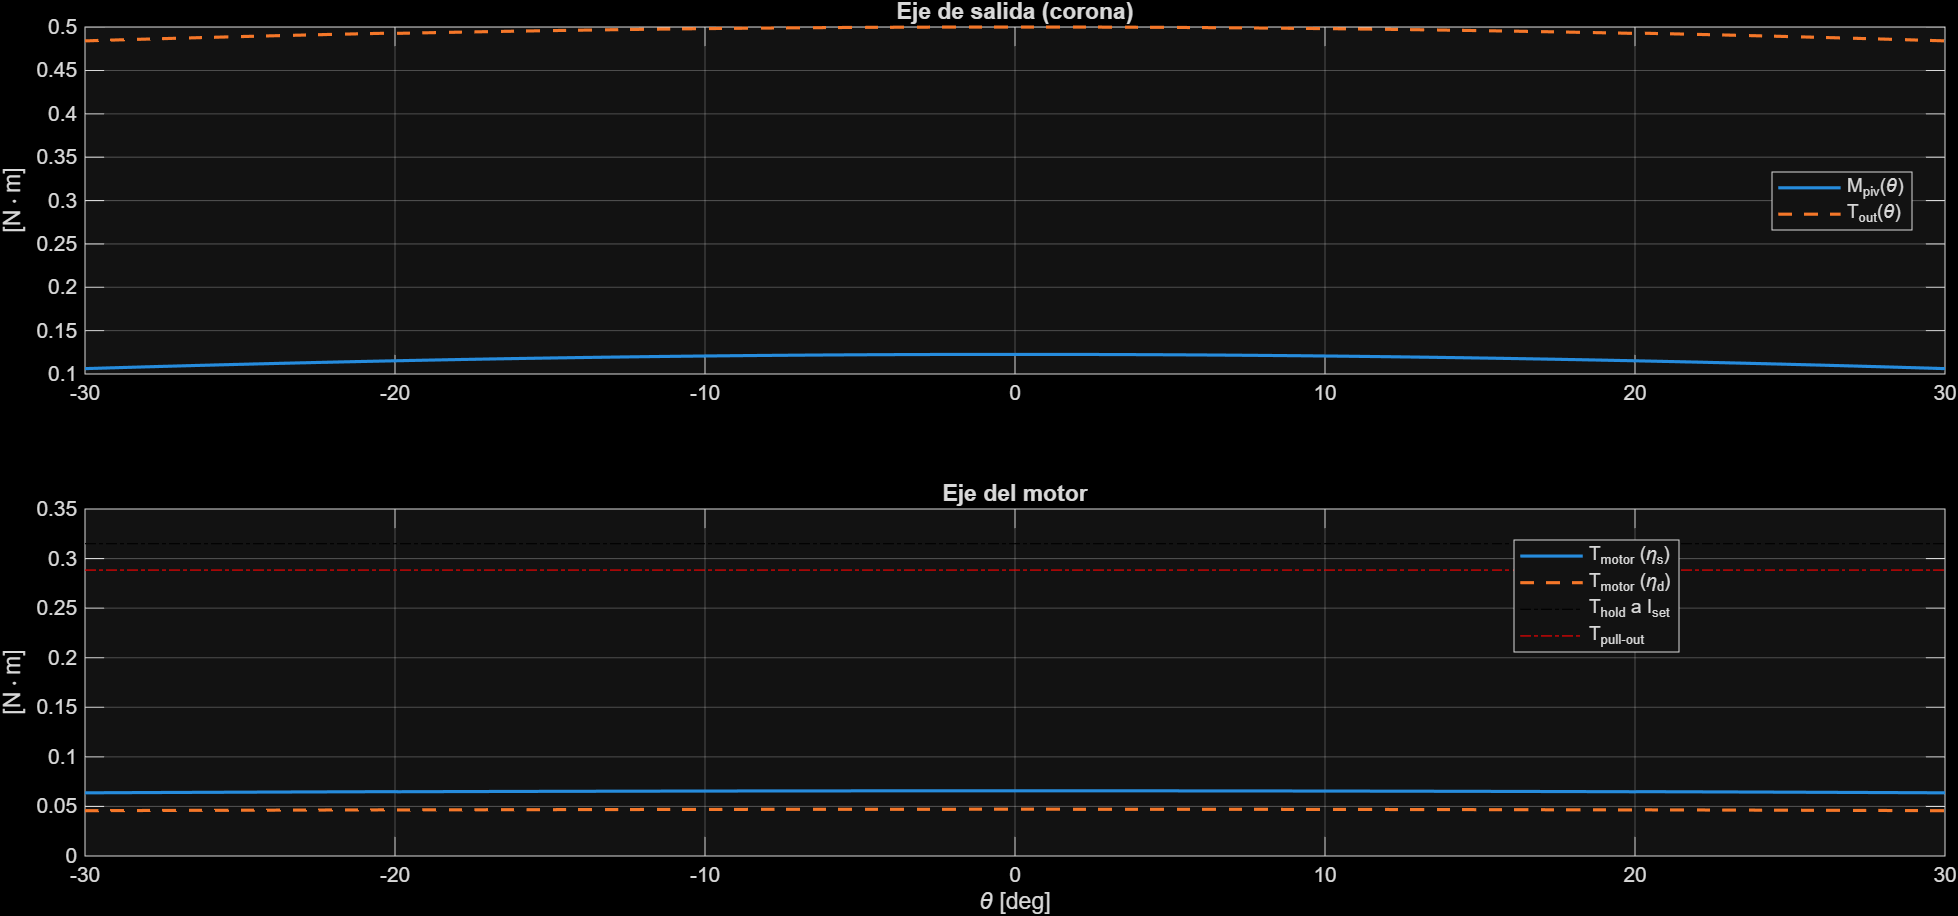
\includegraphics[width=0.85\linewidth]{Recursos/Imagenes/ImagenesDisenoMecanico/Tilt_Torques_MATLAB.png}
	\par\medskip

	\raggedright
	\footnotesize \textit{Nota.} Elaboración propia en MATLAB.
	\label{fig:Torques_Tilt}
\end{figure}

\subsubsection{Esfuerzos en el eje basculante}

La Figura \ref{fig:Eje_Tilt} muestra los diagramas de momento flector y torsor del eje. Entre los rodamientos, el momento flector es pequeño porque la carga de la plataforma entra junto a ellos. El momento crece en el voladizo hasta su máximo de $1.8394\text{ N}\cdot\text{m}$ en el rodamiento derecho. El momento torsor de $0.6502\text{ N}\cdot\text{m}$ actúa solo en el tramo entre la corona y el soporte derecho de la plataforma. Ambos diagramas confirman que la sección crítica es el rodamiento derecho.

\begin{figure}[H]
	\captionsetup{justification=raggedright, singlelinecheck=false, labelsep=none}
	\caption[Diagramas de momento flector y momento torsor en el eje basculante.]{}
	\textit{Diagramas de momento flector y momento torsor en el eje basculante.} \par\medskip

	\centering
	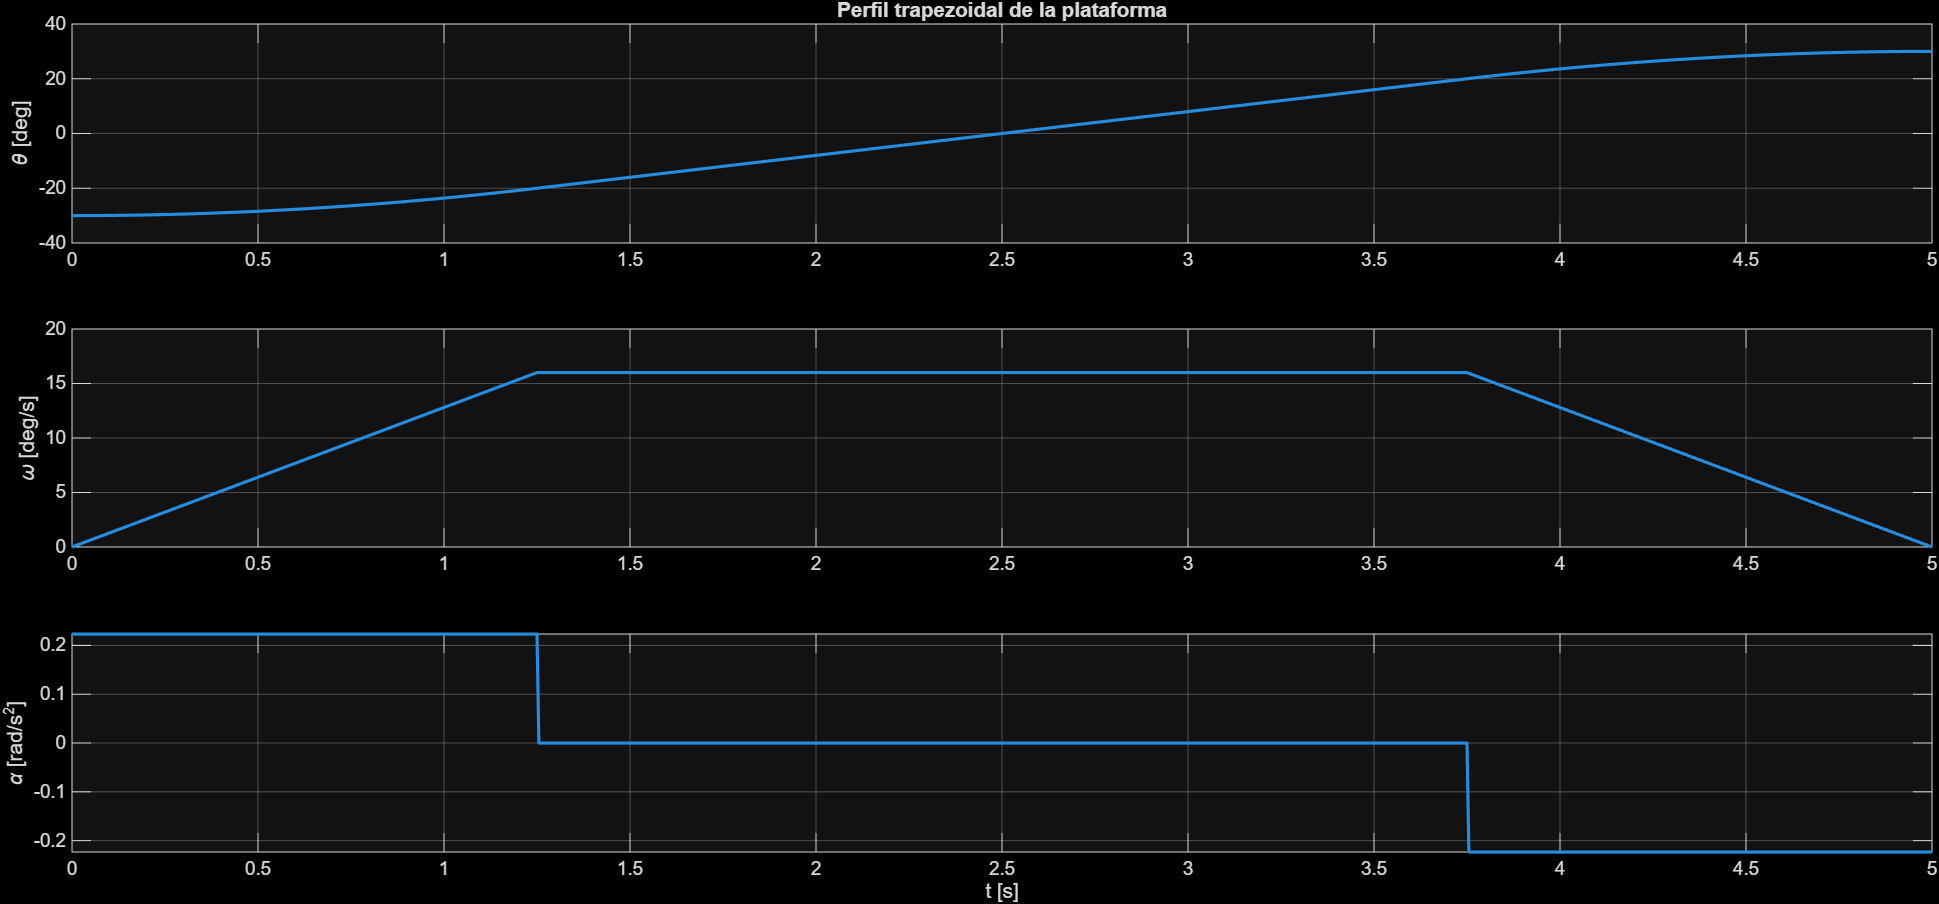
\includegraphics[width=0.85\linewidth]{Recursos/Imagenes/ImagenesDisenoMecanico/Tilt_Eje_MATLAB.png}
	\par\medskip

	\raggedright
	\footnotesize \textit{Nota.} Posición medida desde el centro del rodamiento izquierdo. Elaboración propia en MATLAB.
	\label{fig:Eje_Tilt}
\end{figure}

\subsubsection{Sensibilidad al coeficiente de fricción}

El coeficiente de fricción del contacto entre el sin fin y la corona es el parámetro más incierto del modelo y afecta en sentidos opuestos a dos verificaciones: una fricción alta reduce la eficiencia y aumenta el torque requerido, mientras que una fricción baja reduce el margen de autobloqueo. La Tabla \ref{tab:sensibilidad_mu_tilt} muestra ambos efectos.

\begin{center}
    \footnotesize
    \begin{xltabular}{\textwidth}{|>{\centering\arraybackslash}X|>{\centering\arraybackslash}X|>{\centering\arraybackslash}X|>{\centering\arraybackslash}X|>{\centering\arraybackslash}X|}
        \caption{Sensibilidad de la transmisión al coeficiente de fricción\label{tab:sensibilidad_mu_tilt}} \\
        \hline
        \rowcolor[HTML]{D9E1F2}
        $\mu$ & $\eta$ & Margen de autobloqueo $\mu/\mu_{\text{lím}}$ & $T_{\text{motor}}$ [N$\cdot$m] & FS frente a \textit{pull-out} \\ \hline
        \endfirsthead

        \multicolumn{5}{c}%
        {\tablename\ \thetable{} -- Continuación de la página anterior} \\
        \hline
        \rowcolor[HTML]{D9E1F2}
        $\mu$ & $\eta$ & Margen de autobloqueo $\mu/\mu_{\text{lím}}$ & $T_{\text{motor}}$ [N$\cdot$m] & FS frente a \textit{pull-out} \\ \hline
        \endhead

        \hline
        \endfoot

        \hline
        \endlastfoot

        $0.050$ & $0.598$ & $0.67$ (sin autobloqueo) & $0.0363$ & $7.94$ \\ \hline
        $0.075$ & $0.497$ & $1.00$ (límite) & $0.0436$ & $6.61$ \\ \hline
        $0.087$ (dinámico) & $0.460$ & $1.16$ & $0.0472$ & $6.12$ \\ \hline
        $0.100$ & $0.425$ & $1.33$ & $0.0510$ & $5.66$ \\ \hline
        $0.150$ (diseño) & $0.330$ & $2.00$ & $0.0658$ & $4.38$ \\ \hline
        $0.200$ & $0.269$ & $2.66$ & $0.0808$ & $3.57$ \\ \hline
    \end{xltabular}
\end{center}

En todo el rango analizado, el factor de seguridad del motor frente al \textit{pull-out} se mantiene por encima de $3.5$, por lo que el actuador es adecuado aunque la fricción sea mayor que la de diseño. En cambio, el autobloqueo solo está garantizado en reposo; en movimiento o bajo vibración, el margen puede acercarse a $1$. Este resultado justifica mantener la corriente de retención en el driver y cerrar el lazo de posición con el sensor inercial.

\subsubsection{Presupuesto de error angular}

La resolución del motor no equivale a la precisión del sistema. Con la reducción de 30 a 1, el motor alcanza una resolución de $0.06^\circ$ a paso completo y de $0.00375^\circ$ con 16 micropasos, pero el juego del engrane de $0.28\text{ mm}$ sobre el radio de paso de la corona equivale a un error de $1.070^\circ$. La Tabla \ref{tab:error_angular_tilt} compara la operación en lazo abierto con la operación en lazo cerrado.

\begin{center}
    \footnotesize
    \begin{xltabular}{\textwidth}{|X|>{\centering\arraybackslash}p{3cm}|>{\centering\arraybackslash}p{3cm}|}
        \caption{Presupuesto de error angular de inclinación\label{tab:error_angular_tilt}} \\
        \hline
        \rowcolor[HTML]{D9E1F2}
        Fuente de error & Lazo abierto [$^\circ$] & Lazo cerrado [$^\circ$] \\ \hline
        \endfirsthead

        \multicolumn{3}{c}%
        {\tablename\ \thetable{} -- Continuación de la página anterior} \\
        \hline
        \rowcolor[HTML]{D9E1F2}
        Fuente de error & Lazo abierto [$^\circ$] & Lazo cerrado [$^\circ$] \\ \hline
        \endhead

        \hline
        \endfoot

        \hline
        \endlastfoot

        Juego del engrane & $1.070$ & Compensado \\ \hline
        Resolución del actuador & $0.060$ & $0.00375$ \\ \hline
        Exactitud del sensor inercial & -- & $0.100$ \\ \hline
        Montaje del sensor y de los soportes & $0.200$ & $0.200$ \\ \hline
        Holgura de los rodamientos & $0.050$ & $0.050$ \\ \hline
        Giro por torsión del eje & -- & $0.0177$ \\ \hline
        \textbf{Suma lineal} & $\mathbf{1.380}$ & $\mathbf{0.371}$ \\ \hline
        \textbf{Suma cuadrática (RSS)} & $1.091$ & $0.230$ \\ \hline
        \textbf{Tolerancia IEC 61724-1, Clase A} & $0.5$ & $0.5$ \\ \hline
    \end{xltabular}
\end{center}

En lazo abierto, solo el juego del engrane ya supera la tolerancia de $0.5^\circ$, por lo que el lazo cerrado es indispensable. El sensor inercial está montado en una chapa solidaria al eje, por fuera de la corona; al medir el ángulo del eje, compensa el juego del engrane. Además, por el autobloqueo y la acción de la gravedad, la corona se apoya siempre sobre un mismo flanco. En cambio, el lazo no detecta los errores entre el eje y la plataforma, es decir, el giro por torsión y el montaje de los soportes y del sensor, por lo que estos se mantienen en el presupuesto. La exactitud del sensor inercial corresponde al MPU-6050 tras la calibración de su desviación (\textit{offset}) en el robot \citep{invensense_mpu6050}. Con la suma lineal, que es el criterio más conservador, el error en lazo cerrado es de $0.371^\circ$, por debajo de la tolerancia de $0.5^\circ$.

\subsubsection{Resumen de resultados}

La Tabla \ref{tab:resultados_tilt} resume las verificaciones del subsistema.

\begin{center}
    \footnotesize
    \begin{xltabular}{\textwidth}{|X|>{\centering\arraybackslash}p{2.6cm}|>{\centering\arraybackslash}p{2.6cm}|>{\centering\arraybackslash}p{1.8cm}|}
        \caption{Resumen de verificaciones del subsistema de orientación\label{tab:resultados_tilt}} \\
        \hline
        \rowcolor[HTML]{D9E1F2}
        Verificación & Resultado & Criterio & Estado \\ \hline
        \endfirsthead

        \multicolumn{4}{c}%
        {\tablename\ \thetable{} -- Continuación de la página anterior} \\
        \hline
        \rowcolor[HTML]{D9E1F2}
        Verificación & Resultado & Criterio & Estado \\ \hline
        \endhead

        \hline
        \endfoot

        \hline
        \endlastfoot

        Torque del motor frente a \textit{pull-out} & FS $= 4.39$ & FS $\geq 1$ & Cumple \\ \hline
        Torque del motor frente a retención & FS $= 4.79$ & FS $\geq 1$ & Cumple \\ \hline
        Autobloqueo en reposo ($\mu_s = 0.15$) & $\eta_{\text{inv}} = -0.983$ & $\eta_{\text{inv}} < 0$ & Cumple \\ \hline
        Resistencia del eje a la fluencia & FS $= 8.2$ & FS $\geq 3.0$ & Cumple \\ \hline
        Flecha del eje en la corona & $0.0346\text{ mm}$ & $\leq 0.076\text{ mm}$ & Cumple \\ \hline
        Rodamiento más cargado & $S_0 = 29.3$ & $S_0 \geq 1$ & Cumple \\ \hline
        Prisioneros (par / fuerza axial) & FS $= 11.0$ / $135.3$ & FS $\geq 1$ & Cumple \\ \hline
        Error angular en lazo cerrado & $0.371^\circ$ & $\leq 0.5^\circ$ & Cumple \\ \hline
    \end{xltabular}
\end{center}

El modelo de cálculo tiene limitaciones que deben considerarse al interpretar estos resultados:
\begin{itemize}
    \item supone cuerpos rígidos, salvo para la flecha y la torsión del eje;
    \item suma las cargas como colineales;
    \item adopta valores supuestos para la fricción, el juego del engrane y la exactitud del sensor inercial.
\end{itemize}
Estos valores deben confirmarse en el prototipo midiendo el torque de arranque, el juego del engrane ensamblado y el error de inclinación frente a un inclinómetro de referencia.
% PENDIENTE: agregar el análisis por elementos finitos.

\end{document}